\section{Preliminary Experiments on Mini2048}

% VSE を行うことで性能がどのくらい下がりうるのか,どのように value ranges を設計すればよいかについて
% 知見を得るため,まず 3x3 の mini2048 を用いて評価を行った.
% mini2048 は,3x3 の盤面で行われること以外は2048と同じである.
% すでに完全解析されており,理論的な最高期待値は5469?点だと分かっている.
% 著者らの先行研究において,様々な大きさのN-tupleを設計・実験し,盤面の半分以上をカバーする7タプルまで性能向上が見られることを示した.

We first conducted VSE evaluations using mini2048, a smaller variant of 2048, to gain insight into how much the application of VSE degrades the performance and of which factors of VSE affect performance.
Mini2048 is a smaller variant of 2048 where the game rules are identical to 2048 except that the board size is $3\times 3$.
We chose Mini2048 as the testbed of our preliminary experiments for two reasons: it was strongly solved (a.k.a. perfectly analyzed)~\cite{YaKN22,TeKM23} and the expected score of the optimal play is known to be 5468.49; we confirmed in our previous work~\cite{TeMa25} that enlarging the size of the N-tuple yielded better performance up to 6-tuples.

% 実験では,m-NT6 を例にとり,複数の value ranges の組合せによる VSE を行ったときのプレイヤの性能を調べる.
% ここでは,最大3つに分割する VSE を複数試す.ここで調べたいことは以下の3つである.
%  - VSE を行うことで,どのくらいの性能低下がありうるか.
%  - 分割にあたって,複数の分割に含まれるバッファを持たせるべきか.
%  - VSE を行ったときに,性能に最も影響する要素は何か.

\begin{table}
 \caption{N-tuple networks used for mini2048.}
 \label{table:mNT}
 \centering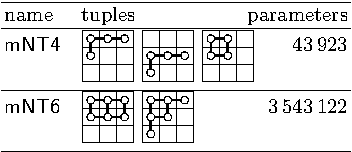
\includegraphics[]{figures/mNT-table.pdf}
\end{table}

In preliminary experiments, we used two manually designed N-tuple networks in Table~\ref{table:mNT}: \textsf{mNT6} with two 6-tuples and \textsf{mNT4} with three 4-tuples. We applied multiple VSEs on \textsf{mNT6}.
The main questions that we wanted to examine were the following:
\begin{itemize}
 \item To what extent does VSE degrade performance?
 \item Should we have overlaps between value ranges when splitting?
 \item Which factor of VSE affects performance most strongly?
\end{itemize}


% 比較として,VSE を行わない m-NT4 の結果も示す.
% 学習は,OI=1200 で初期化したTC学習とし,$5\times10^8$ steps だけ学習させる.
% 10個の異なるseedsを用いた学習から得られる10個のプレイヤにgreedy に??ゲームプレイさせたときの平均得点を調べる.

For each configuration, we trained N-tuple networks using Temporal Coherence learning with Optimistic Initialization~\cite{GuCW22} (initial value 1200) for $5\times 10^8$ steps.  After the training, we played 1\,000 games with 1-ply lookahead (the greedy play) and evaluated the performance in terms of the average score.  To mitigate the effect of randomness, we conducted each training with 10 different random seeds.
Table~\ref{table:pre-results} summarizes the configurations of VSEs and the average score of the trained N-tuple networks.

\begin{table}
\caption{Configurations of preliminary experiments for mini2048 and the average score for 1000 games with the 1-ply lookahead. The numbers in parentheses after value ranges show the number of possible values after the corresponding mapping. For average scores, the mean and standard deviation over 10 training runs are given (after the $\pm$ sign).}
\label{table:pre-results}
 \setlength{\doublerulesep}{.4pt}
 \centering\begin{tabular}{l|l|p{170pt}|r|r}
  \hline\hline
   tuple			& VSE			& value ranges									& parameters	& ave. score \\
  \hline
% (* 11 11 11 11 11 11 1 2)3543122
   \multirow{11}{*}{\textsf{mNT6}}	& \mbox{no VSE}		& \phantom{\rule{1pt}{9.5pt}}$2^1$--$2^{10}$\,(11)								& 3\,543\,122	& 4\,610.2$\pm$\phantom{0}81.1 \\ \cline{2-5}
% (* 8 8 8 8 8 8 2 2)1048576
				& \mbox{2-VSE-A}	& \phantom{\rule{1pt}{9.5pt}}$2^1$--$2^6$\,(8), $2^{5}$--$2^{10}$\,(8)					& 1\,048\,576	& 4\,555.8$\pm$\phantom{0}91.7\\ \cline{2-5}
% (+ (* 8 8 8 8 8 8 1 2) (* 7 7 7 7 7 7 1 2))759586
				& \mbox{2-VSE-B}	& \phantom{\rule{1pt}{9.5pt}}$2^1$--$2^6$\,(8), $2^{6}$--$2^{10}$\,(7)					& 759\,586	& 4\,584.0$\pm$\phantom{0}69.9\\ \cline{2-5}
% (+ (* 8 8 8 8 8 8 1 2) (* 6 6 6 6 6 6 1 2))617600
				& \mbox{2-VSE-C}	& \phantom{\rule{1pt}{9.5pt}}$2^1$--$2^6$\,(8), $2^{7}$--$2^{10}$\,(6)					& 617\,600	& 4\,557.3$\pm$\phantom{0}74.5\\ \cline{2-5}
% (+ (* 7 7 7 7 7 7 2 2))470596
				& \mbox{2-VSE-D}	& \phantom{\rule{1pt}{9.5pt}}$2^1$--$2^5$\,(7), $2^{6}$--$2^{10}$\,(7)					& 470\,596	& 4\,621.1$\pm$\phantom{0}83.5\\ \cline{2-5}
% (+ (* 6 6 6 6 6 6 1 2) (* 8 8 8 8 8 8 1 2))617600
				& \mbox{2-VSE-E}	& \phantom{\rule{1pt}{9.5pt}}$2^1$--$2^4$\,(6), $2^{5}$--$2^{10}$\,(8)					& 617\,600	& 4\,441.4$\pm$\phantom{0}96.7\\ \cline{2-5}
% (+ (* 6 6 6 6 6 6 2 2) (* 5 5 5 5 5 5 1 2))217874
				& \mbox{3-VSE-A}	& \phantom{\rule{1pt}{9.5pt}}$2^1$--$2^4$\,(6), $2^{5}$--$2^{7}$\,(6), $2^8$--$2^{10}$\,(5)			& 217\,874	& 4\,390.9$\pm$111.6\\ \cline{2-5}
% (+ (* 6 6 6 6 6 6 2 2) (* 7 7 7 7 7 7 1 2))
				& \mbox{3-VSE-B}	& \phantom{\rule{1pt}{9.5pt}}$2^1$--$2^4$\,(6), $2^{4}$--$2^{7}$\,(7), $2^7$--$2^{10}$\,(6)			& 421\,922	& 4\,464.9$\pm$\phantom{0}64.7\\ \cline{2-5}
% (+ (* 6 6 6 6 6 6 1 2) (* 5 5 5 5 5 5 2 2) (+ 4 4 4 4 4 4 1 2))155839
				& \mbox{4-VSE-A}	& \phantom{\rule{1pt}{9.5pt}}$2^1$--$2^4$\,(6), $2^5$--$2^6$\,(5), $2^7$--$2^8$\,(5), $2^9$--$2^{10}$\,(4)	& 155\,839	& 4\,451.7$\pm$\phantom{0}96.7\\ \hline
   \textsf{mNT4}				& \mbox{no VSE}		& \phantom{\rule{1pt}{9.5pt}}$2^1$--$2^{10}$\,(11)								& 43\,923	& 3\,226.0$\pm$141.4\\\hline
 \end{tabular}
\end{table}

% 表より,とても promissing な結果が得られた.
% VSE を行うことで,性能低下は起こりうるが,m-NT4 との比較からタプルサイズ拡大による性能向上を打ち消すほどではない.
% 分割の際に,複数の分割に共通の値が含まれるようなバッファを用いる必要はない.
% これは,著者らの当初の想定に反する結果であった.
% 性能に最も影響するのは,一番小さなrangeに含まれる要素数である.
% 一番小さな range に含まれる要素数が同じであれば,それより上のrangeをさらに分割してもしなくても大差ないようだ.

The results in Table~\ref{table:pre-results} were very promising.
All the results from \textsf{mNT6} plus VSEs outperformed those of \textsf{mNT4}.
Although the application of VSE degrades performance (for the case of \textsf{mNT6}, $<$5\%) in general, the N-tuple networks with 2-VSE-D were slightly better than the original \textsf{mNT6} without VSE.
From the results of 2-VSE-A, 2-VSE-B and 2-VSE-C, as well as 3-VSE-A and 3-VSE-B, we found that it was not necessary to introduce overlaps between the value ranges; this was contrary to the initial assumption of the authors.
The factor with the greatest impact on performance was the number of elements included in the smallest value range as seen in 2-VSE-C, 2-VSE-D, and 2-VSE-E
If the size of the smallest range was the same, then further splitting of higher ranges appeared to make little difference as seen in 2-VSE-E, 3-VSE-A, and 4-VSE-A.

We will use these findings in the design of the VSEs for the original 2048.

% LocalWords:  VSE testbed mNT VSEs lookahead
